\documentclass[tikz]{standalone}
\usetikzlibrary{patterns}
\begin{document}
  \tikzset{>=latex} % Change default arrowhead to filled triangle
  \def\stencil[#1, #2]{% x, y
    \draw[very thick, red] (#1+1, #2) rectangle (#1+2, #2-3);
    \draw[very thick, red] (#1, #2-1) rectangle (#1+3, #2-2);
  }

  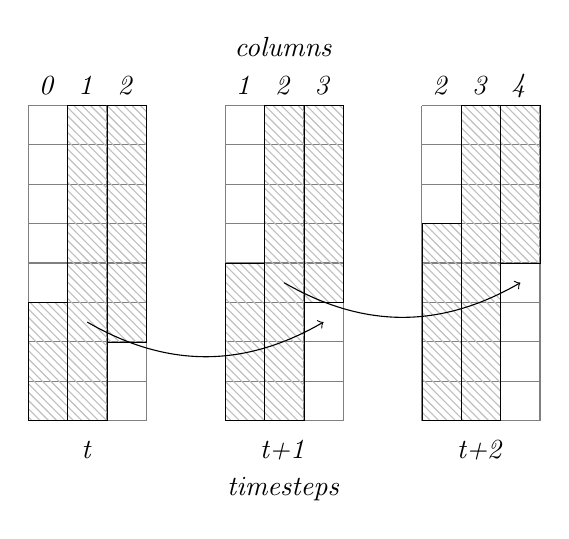
\begin{tikzpicture}[scale=0.5]

    \draw[gray, step=1] (0,0) grid (3,8);
    \node at(0.5, 8.5) {\emph{0}}; \node at(1.5, 8.5) {\emph{1}}; \node at(2.5, 8.5) {\emph{2}};
    \draw[pattern color=lightgray, pattern=north west lines, very thin](0, 0) rectangle (1, 3);
    \draw[pattern color=lightgray, pattern=north west lines, very thin](1, 0) rectangle (2, 8);
    \draw[pattern color=lightgray, pattern=north west lines, very thin](2, 2) rectangle (3, 8);
    \node at(1.5, -0.75) {\emph{t}};
    \stencil[0, 4]
    
    \draw[gray, step=1] (5,0) grid (8,8);
    \node at(6.5, 9.5) {\emph{columns}};
    \node at(5.5, 8.5) {\emph{1}}; \node at(6.5, 8.5) {\emph{2}}; \node at(7.5, 8.5) {\emph{3}};
    \draw[pattern color=lightgray, pattern=north west lines, very thin](5, 0) rectangle (6, 4);
    \draw[pattern color=lightgray, pattern=north west lines, very thin](6, 0) rectangle (7, 8);
    \draw[pattern color=lightgray, pattern=north west lines, very thin](7, 3) rectangle (8, 8);
    \node at(6.5, -0.75) {\emph{t+1}};
    \node at(6.5, -1.75) {\emph{timesteps}};
    \stencil[5, 5]

    \draw[gray, step=1] (10,0) grid (13,8);
    \node at(10.5, 8.5) {\emph{2}}; \node at(11.5, 8.5) {\emph{3}}; \node at(12.5, 8.5) {\emph{4}};
    \draw[pattern color=lightgray, pattern=north west lines, very thin](10, 0) rectangle (11, 5);
    \draw[pattern color=lightgray, pattern=north west lines, very thin](11, 0) rectangle (12, 8);
    \draw[pattern color=lightgray, pattern=north west lines, very thin](12, 4) rectangle (13, 8);
    \node at(11.5, -0.75) {\emph{t+2}};
    \stencil[10, 6]

    % Communications arrows
    \path[->]
    (1.5, 2.5) edge[bend right] (7.5, 2.5)
    (6.5, 3.5) edge[bend right] (12.5, 3.5);

  \end{tikzpicture}
\end{document}
